% !TEX root = ../tfg.tex

Este capítulo presenta cómo se comporta el sistema cuando se mide con datos.
Primero se evalúa cada componente por separado y después el sistema completo, en el que cada etapa recibe lo que produce la anterior.
A estas medidas se suma el tiempo que tarda el sistema en procesar un punto y una lectura conjunta de todos los resultados.
Con ello se comprueba hasta qué punto se cumplen los objetivos planteados en el \cref{cap:introduccion}.

Todas las cifras se miden sobre una muestra limitada de puntos y de torneos, de modo que no puede asumirse que con otros datos salgan igual.
Para saber cuánto podrían variar, las cifras principales se acompañan de una medida de su incertidumbre.
En la mayoría de los casos se trata de un intervalo de confianza del 95~\%, que estima cuánto cambiaría la cifra si se repitiera la medida con otros puntos.
El detector de sonido es la excepción, porque su incertidumbre se mide con la desviación típica de tres entrenamientos, tal como se explica en su apartado.

Estos intervalos se calculan con el método \textit{bootstrap}~\cite{efron1979bootstrap}, que se aproxima mediante un método de Monte Carlo con \num{10000} remuestreos.
Ambos se explican en la \cref{sec:fund-evaluacion}.

\section{Resultados de cada componente}
\label{sec:resultados-componentes}

Para saber cuánto vale cada componente conviene medirlo por separado, con datos anotados y sin que le lleguen los errores de los demás.
El orden en el que se explican los resultados de cada componente es el mismo en el que el sistema procesa los puntos.

\subsection{Instante del golpe}
\label{sec:resultados-instante}

El detector de golpes por sonido se evalúa con los 99 puntos de CVSPORTS, de los que se conoce el instante de cada uno de sus 2377 golpes.
Los puntos se reparten de forma aleatoria en dos grupos, uno de 70 puntos para entrenar la red y otro de 29 para medirla.

Un reparto aleatorio tiene el inconveniente de que puede resultar más fácil o más difícil de lo normal, según los puntos que queden en cada grupo.
Por eso el entrenamiento se repite tres veces, cada una con su propio reparto y con sus propios pesos iniciales.
La cifra final es la media de las tres ejecuciones y se acompaña de su desviación típica, que indica cuánto varía el resultado de una ejecución a otra.

Para decidir si una detección es correcta hay que compararla con las anotaciones.
Se considera que un golpe se ha detectado bien cuando el sistema señala un instante a menos de 250~ms de uno anotado, y cada golpe anotado solo puede emparejarse con una detección.
Esta segunda condición evita que una misma detección cuente como acierto para varios golpes.

Con este criterio el F1 medido es de 0,958 $\pm$ 0,007, con una precisión de 0,972 y un \textit{recall} de 0,945 (\cref{tab:audio-ejecuciones}).
La precisión es mayor que el \textit{recall}, y eso indica que casi todas las detecciones corresponden a golpes reales y que la mayor parte de los errores son golpes que el sistema no llega a detectar.

\begin{table}[htbp]
  \centering
  \caption{Resultado del detector de golpes por sonido: media de las tres ejecuciones y desviación típica del F1.}
  \label{tab:audio-ejecuciones}
  \small
  \begin{tabular}{lccc}
\toprule
\textbf{Resultado} & \textbf{Precisión} & \textbf{\textit{Recall}} & \textbf{F1} \\
\midrule
Media de tres ejecuciones & \num{0.972} & \num{0.945} & \num{0.958} $\pm$ \num{0.007} \\
\bottomrule
\end{tabular}

\end{table}

\subsection{Pelota}
\label{sec:resultados-pelota}

La pelota se evalúa con la final femenina del conjunto PadelTracker100 que la red no ha visto durante el entrenamiento (\cref{sec:padeltracker}).

Para decidir si una detección es correcta se compara su posición con la que consta en las
anotaciones.
Si esta posición se encuentra a menos de 15 píxeles de la pelota anotada se considera un acierto.
Esta tolerancia es algo mayor que el lado de una celda del mapa de calor, que equivale a 10 píxeles, y deja un margen razonable para el error propio de la red.

Con este criterio el F1 medido es de 0,915, con una precisión de 0,871 y un \textit{recall} de 0,964.
Además, el error mediano de la posición es de 8,1 píxeles.

Estos resultados tienen una limitación que conviene reconocer.
Las dos finales se jugaron en la misma pista y con la misma cámara, de modo que no pueden demostrar cómo se comportaría el detector en otras condiciones.
La evaluación del sistema completo aporta una comprobación parcial, porque allí la pelota se detecta en torneos con pistas y cámaras que la red no ha visto (\cref{sec:sistema-completo}).

\subsection{Asignación del golpe}
\label{sec:resultados-asignacion}

La asignación se evalúa con los 16 puntos de Vigo en los que se indica qué jugador ejecuta cada golpe.
Son los únicos puntos del conjunto con esa información, y por eso la medida se apoya en un solo torneo.

Para medir solo este componente se utilizan los instantes anotados y no los que detecta el sonido.
De este modo los errores del detector no afectan a la medida, que refleja únicamente lo bien que el sistema atribuye cada golpe al jugador que lo ejecuta.

Se mide además si el sistema acierta la pareja cuando el jugador asignado pertenece al mismo equipo que el que golpea.
Esta medida se incluye porque es la que ofrecen también Decorte \textit{et al.} y permite comparar con ellos.
Para HAT, sin embargo, la cifra que realmente importa es la del jugador.
Si el golpe no se atribuye al jugador exacto no puede conocerse su tipo, porque el clasificador analizaría el movimiento de otra persona, y tampoco puede contarse en las estadísticas de quien lo ejecutó.
Es por ello que acertar solo la pareja no es una métrica válida para los fines de HAT.

Como muestra la \cref{tab:asignacion-paper}, el sistema acierta el jugador en el 87,5~\% de los golpes y la pareja en el 92,2~\%, lo que supone 3,8 y 5,4 puntos más que el resultado de Decorte \textit{et al.} sobre esos mismos golpes.
Los intervalos de confianza para esta comparación son anchos, de entre 12 y 15 puntos.
Esto se debe a que la medida se apoya en un solo torneo y en un número pequeño de puntos.

\begin{table}[htbp]
  \centering
  \caption{Acierto de la asignación del golpe frente a Decorte \textit{et al.}\ en los mismos golpes.}
  \label{tab:asignacion-paper}
  \begin{tabular}{lcccc}
\toprule
\textbf{Acierto} & \textbf{Este trabajo} & \textbf{Intervalo 95~\%} & \textbf{Decorte \textit{et al.}} & \textbf{Diferencia} \\
\midrule
Jugador & \SI{87.5}{\percent} & \num{78.4}--\num{93.6} & \SI{83.7}{\percent} & \num[retain-explicit-plus]{+3.8} \\
Pareja & \SI{92.2}{\percent} & \num{84.4}--\num{96.8} & \SI{86.8}{\percent} & \num[retain-explicit-plus]{+5.3} \\
\bottomrule
\end{tabular}

\end{table}

Para saber si esa diferencia es concluyente no es suficiente con comparar las dos cifras, porque cada una tiene su propia incertidumbre.
Para ello, se calcula el intervalo de la diferencia con el mismo \textit{bootstrap}, eligiendo en cada remuestreo los mismos puntos para los dos métodos.
Así la dificultad de cada punto afecta por igual a ambos y se cancela en la comparación.

El intervalo de la diferencia va de $-5{,}4$ a 9,9 puntos para el jugador y de $-2{,}9$ a 10,2 para la pareja.
Como los dos incluyen el cero, no puede afirmarse que el sistema supere a Decorte \textit{et al.}, aunque queda por encima en media.
Lo que sí se sostiene es que la réplica de su método alcanza un acierto al menos comparable al suyo.

\subsection{Tipo de golpe}
\label{sec:resultados-tipo}

El clasificador se evalúa con el etiquetado propio.

Sin embargo, no todos los golpes etiquetados pueden utilizarse.
Es necesario descartar los 167 que se anotaron como ``otro'', que no se emplean ni para entrenar ni para evaluar (\cref{sec:etiquetado}), y otros 24 en los que no hay un jugador asignado o en los que el jugador falta en la mayor parte de la ventana, de modo que el modelo no tiene un movimiento que analizar, dejando en total 2186 golpes.

Para repartir esos golpes entre entrenamiento y evaluación no es suficiente con hacerlo al azar.
La razón de esto es que los puntos de un mismo torneo comparten pista, cámara e iluminación, y si se mezclaran el modelo podría entrenar con la misma pista con la que después se evalúa, lo que daría un resultado optimista.
Por esta razón, se deja un torneo fuera cada vez, de modo que se entrena con diez y se mide en el que falta, y esto se repite once veces.
Así la evaluación muestra cómo funciona el clasificador en una pista y una cámara que nunca ha visto.

Con este protocolo el acierto global, medido con el \textit{accuracy}, es del 82,7~\%, con un intervalo de confianza que va del 80,3~\% al 85,0~\%.
El intervalo se calcula remuestreando torneos completos y no golpes sueltos.
La segunda medida es el macro-F1, que es la media del F1 de las cuatro clases y hace que todas pesen igual aunque tengan un número muy distinto de ejemplos.
Su valor es de 0,859.

El resultado varía considerablemente de un torneo a otro, como muestra la \cref{tab:tipo-torneos}.
El acierto va del 75,4~\% de Ámsterdam al 91,7~\% de Malmö, una diferencia de más de 16 puntos.
Esto indica que la dificultad no es la misma en todas las pistas, y que la cifra global es un promedio de situaciones distintas.

\begin{table}[htbp]
  \centering
  \caption{\textit{Accuracy} del clasificador en cada torneo, dejándolo fuera del entrenamiento.}
  \label{tab:tipo-torneos}
  \small
  \begin{tabular}{lc}
    \toprule
    Torneo & \textit{Accuracy} (\%) \\
    \midrule
    Malmö & 91,7 \\
    Málaga & 86,2 \\
    Alemania & 85,8 \\
    Vigo & 84,7 \\
    Finlandia & 83,4 \\
    Menorca & 83,1 \\
    Valladolid & 81,1 \\
    Madrid & 80,5 \\
    Bruselas & 78,5 \\
    Valencia & 76,3 \\
    Ámsterdam & 75,4 \\
    \bottomrule
  \end{tabular}
\end{table}

Los resultados por clase se recogen en la \cref{tab:tipo-clases}.
El saque y el remate son las clases que mejor se reconocen, con un F1 de 0,956 y de 0,879 respectivamente.
La derecha y el revés están en torno a 0,80, y son además las dos clases con más ejemplos.

\begin{table}[htbp]
  \centering
  \caption{Resultados del clasificador por tipo de golpe, dejando fuera un torneo cada vez.}
  \label{tab:tipo-clases}
  \begin{tabular}{lcccc}
\toprule
\textbf{Clase} & \textbf{Precisión} & \textbf{\textit{Recall}} & \textbf{F1} & \textbf{Golpes} \\
\midrule
Derecha & \num{0.806} & \num{0.804} & \num{0.805} & \num{799} \\
Revés & \num{0.789} & \num{0.803} & \num{0.796} & \num{731} \\
Remate & \num{0.882} & \num{0.877} & \num{0.879} & \num{561} \\
Saque & \num{1.000} & \num{0.916} & \num{0.956} & \num{95} \\
\midrule
Media (macro) &  &  & \num{0.859} & \num{2186} \\
\bottomrule
\end{tabular}

\end{table}

La matriz de confusión de la \cref{fig:tipo-confusion} muestra dónde se equivoca el clasificador.
El 63~\% de sus errores son confusiones entre la derecha y el revés, y otro 35~\% confunden el remate con alguno de los dos.
Los saques mal clasificados suponen apenas el 2~\% restante.

\begin{figure}[htbp]
  \centering
  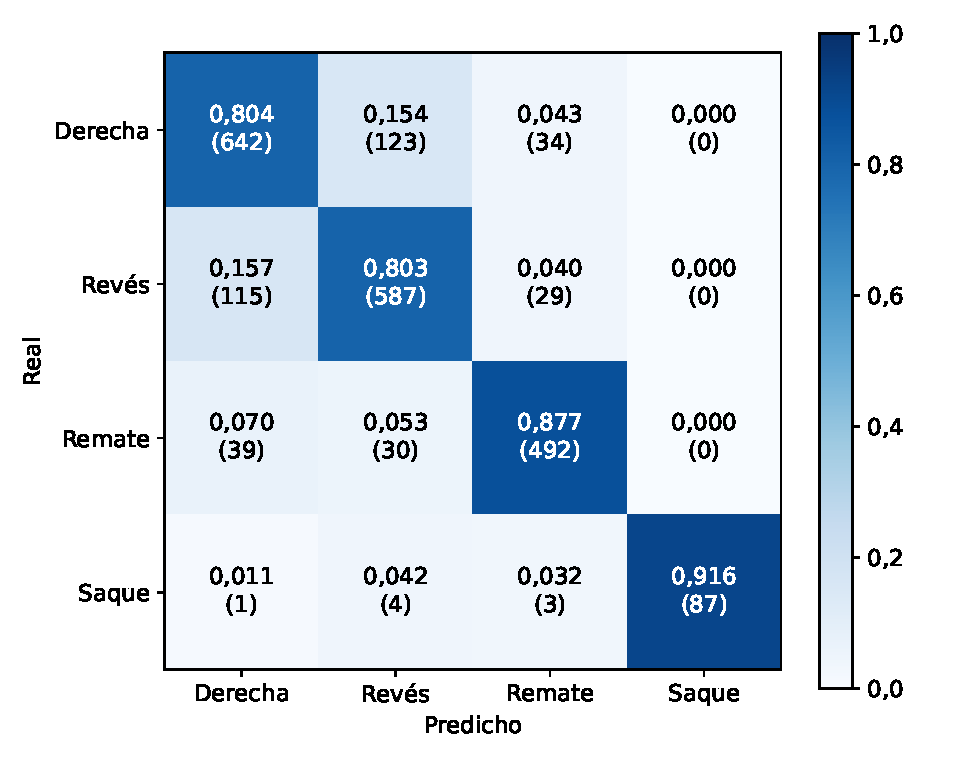
\includegraphics[width=0.7\textwidth]{figuras/matriz-confusion}
  \caption{Matriz de confusión del clasificador de tipo de golpe. Cada casilla indica la proporción de su fila y, entre paréntesis, el número de golpes.}
  \label{fig:tipo-confusion}
\end{figure}

La regla del saque, descrita en la \cref{sec:salida-clasificador}, mejora estos resultados.
Elimina 14 saques falsos que el modelo predecía en mitad del punto, con lo que la precisión del saque pasa de 0,861 a 1,000 sin perder ningún saque real, porque el \textit{recall} se mantiene en 0,916.
El macro-F1 sube así de 0,842 a 0,859 y el \textit{accuracy} del 82,5~\% al 82,7~\%.
Conviene señalar que esta mejora procede del reglamento del pádel y no del aprendizaje del modelo, ya que la regla se limita a descartar lo que el juego no permite.

Para compensar que el saque tiene muy pocos ejemplos se probó también a darle más peso durante el entrenamiento.
Los resultados fueron ligeramente inferiores a los de entrenar sin pesos, y por eso se mantuvo el entrenamiento sin ellos.

\section{El sistema completo}
\label{sec:sistema-completo}

Una vez evaluados los componentes de forma individual, se procede a analizar el sistema completo, de extremo a extremo.
Frente a la evaluación aislada, cada componente trabaja ahora con la salida del anterior y no con datos anotados, por lo que este análisis mide lo que realmente entrega el sistema.
En la práctica, esto implica que los errores de cada fase se transmiten a las siguientes: un golpe no detectado no puede asignarse, y uno asignado al jugador equivocado se clasifica con el esqueleto de otro.

El protocolo de evaluación es el mismo que el del clasificador, con un matiz que lo hace más exigente.
Se deja un torneo fuera cada vez, pero ahora en cada ronda se vuelven a entrenar sin él tanto el detector de sonido como el clasificador, que son los dos componentes que aprenden de CVSPORTS.
La postura y la pelota no se entrenaron con este conjunto, de modo que ningún modelo del sistema ha visto el torneo con el que se mide.
Gracias a ello el resultado refleja lo que ocurriría al aplicar el sistema a una pista nueva.

La \cref{tab:cadena} recoge el resultado de este experimento.
Para cada etapa indica el porcentaje de golpes reales que la superan junto con todas las anteriores, de modo que cada fila incluye los fallos de las filas que tiene encima.
La tabla se divide en dos bloques porque no todos los datos permiten medir lo mismo.
Los 11 torneos sirven para comprobar la detección y el tipo, pero solo Vigo tiene anotado el jugador que ejecuta cada golpe, y por eso es el único donde puede medirse la cadena completa.

\begin{table}[htbp]
  \centering
  \caption{Sistema completo por etapas: porcentaje de golpes reales que superan cada etapa y todas las anteriores.}
  \label{tab:cadena}
  \begin{tabular}{lcc}
\toprule
\textbf{Golpes que el sistema:} & \textbf{\%} & \textbf{Intervalo 95~\%} \\
\midrule
\multicolumn{3}{@{}l}{\emph{Los 11 torneos (2210 golpes)}} \\
Detecta & \num{96.0} & \num{94.9}--\num{97.0} \\
Detecta y clasifica bien & \num{80.1} & \num{77.4}--\num{82.6} \\
\midrule
\multicolumn{3}{@{}l}{\emph{Vigo, con el jugador anotado (286 golpes)}} \\
Detecta & \num{96.2} & \num{93.8}--\num{98.3} \\
Detecta y asigna al jugador correcto & \num{84.6} & \num{76.3}--\num{90.9} \\
Detecta, asigna al jugador correcto y clasifica bien & \num{75.5} & \num{66.9}--\num{82.2} \\
\bottomrule
\end{tabular}

\end{table}

En Vigo el sistema detecta el 96,2~\% de los golpes, de ellos el 84,6~\% son asignados al jugador correcto y el 75,5~\% lo hace con la clase correcta, de modo que tres de cada cuatro golpes son correctos.
La caída entre una etapa y la siguiente indica dónde se pierde más.
La detección deja fuera apenas unos 4 puntos, mientras que la asignación pierde casi 12 y la clasificación algo más de 9.
La etapa más débil de la cadena es, por tanto, la asignación del golpe al jugador.

En el conjunto de los 11 torneos el sistema detecta el 96,0~\% de los golpes y acierta además el tipo en el 80,1~\%, es decir, cuatro de cada cinco golpes se detectan y se clasifican bien.
Estos 2210 golpes son los que se han etiquetado con una de las cuatro clases.
A diferencia de la evaluación del clasificador, que usa 2186, aquí también cuentan como fallo los 24 golpes que no pueden clasificarse porque no tienen jugador asignado.
La tabla solo cuenta golpes reales y no refleja las detecciones falsas, que son las que el sistema señala sin que haya ningún golpe.
Estas suponen apenas el 2,8~\% de todas las detecciones, por lo que añaden pocos golpes inexistentes a las estadísticas.

\section{Coste de procesado}
\label{sec:coste}

Además de cuánto acierta, interesa conocer cuánto tarda el sistema en procesar un punto.
Como referencia, se compara con la duración del propio punto.
Medirlo exige indicar primero con qué equipo se ha hecho, porque el resultado depende de él.

El equipo utilizado, tanto para entrenar los modelos como para medir el tiempo, es un ordenador de sobremesa cuyas características recoge la \cref{tab:equipo}.
Su elemento más relevante es la tarjeta gráfica, porque es la que ejecuta los modelos de postura y de pelota, que son los más costosos del sistema.
Se trata de un equipo de consumo y no de un servidor especializado.

\begin{table}[htbp]
  \centering
  \caption{Equipo con el que se ha medido el coste de procesado.}
  \label{tab:equipo}
  \begin{tabular}{ll}
\toprule
\textbf{Componente} & \textbf{Especificación} \\
\midrule
Tarjeta gráfica & NVIDIA GeForce RTX 3090, 24~GB \\
Procesador & AMD Ryzen 9 5900X, 12 núcleos y 24 hilos \\
Memoria RAM & 32~GB \\
Sistema operativo & Windows 11 Pro con WSL2 (Ubuntu 26.04 LTS) \\
Software & Python 3.11.15, PyTorch 2.13.0 (CUDA 13.0) \\
\bottomrule
\end{tabular}

\end{table}

La medida se realizó sobre un punto real, el VIGO\_11, que dura 64,3~s en un vídeo de 1080p a 25~\ac{fps}.
Procesarlo por completo con el sistema tarda 67,5~s, es decir, 1,05 veces la duración del vídeo.

La \cref{tab:coste} desglosa ese tiempo por etapas.
El mayor coste corresponde a la postura de los jugadores y a la detección de la pelota, que juntas suponen cerca del 80~\% del total.
Son las dos etapas que procesan la imagen fotograma a fotograma con una red neuronal, y por eso requieren mucho más cálculo que el resto.

\begin{table}[htbp]
  \centering
  \caption{Tiempo de procesado de un punto, por etapa.}
  \label{tab:coste}
  \begin{tabular}{lcc}
\toprule
\textbf{Etapa} & \textbf{Tiempo} & \textbf{Parte del total} \\
\midrule
Audio: detección del golpe & \SI{0.2}{\second} & \SI{0.3}{\percent} \\
Postura de los jugadores & \SI{27.1}{\second} & \SI{40.2}{\percent} \\
Pelota & \SI{26.3}{\second} & \SI{39.0}{\percent} \\
Resto: lectura del vídeo, identidad, asignación y tipo & \SI{13.8}{\second} & \SI{20.5}{\percent} \\
\midrule
Total & \SI{67.5}{\second} &  \\
\bottomrule
\end{tabular}

\end{table}

En el extremo contrario está el audio, donde el detector de golpes por sonido tarda 0,2~s, menos del 1~\% del tiempo de cómputo total.
El resto del tiempo, un 20,5~\%, se reparte entre la lectura del vídeo, la identidad de los jugadores, la asignación de cada golpe y la clasificación de su tipo.
Ninguna de estas tareas destaca por sí sola, y su suma es menor que cualquiera de las dos etapas principales.

Hay una parte del proceso que esta medida no incluye, y es la generación del vídeo con la información dibujada encima.
Se realiza en una segunda pasada opcional, porque no forma parte del análisis sino de su comprobación visual.

Estas medidas corresponden a un único punto y a un único equipo, de modo que deben tomarse como una referencia del orden de magnitud y no como una cifra general.
